\documentclass{article}

\usepackage{graphicx}
\usepackage{tikz}
\usepackage{tikzsymbols}
\usetikzlibrary{calc,patterns,shapes.geometric}
\pagestyle{empty}
\usepackage[margin=0pt]{geometry}
\geometry{papersize={14in,12in}}

\def\centerarc[#1](#2)(#3:#4:#5){\draw[#1] ($(#2)+({#5*cos(#3)},{#5*sin(#3)})$) arc (#3:#4:#5);}

\begin{document}
	\begin{figure}
		\centering
		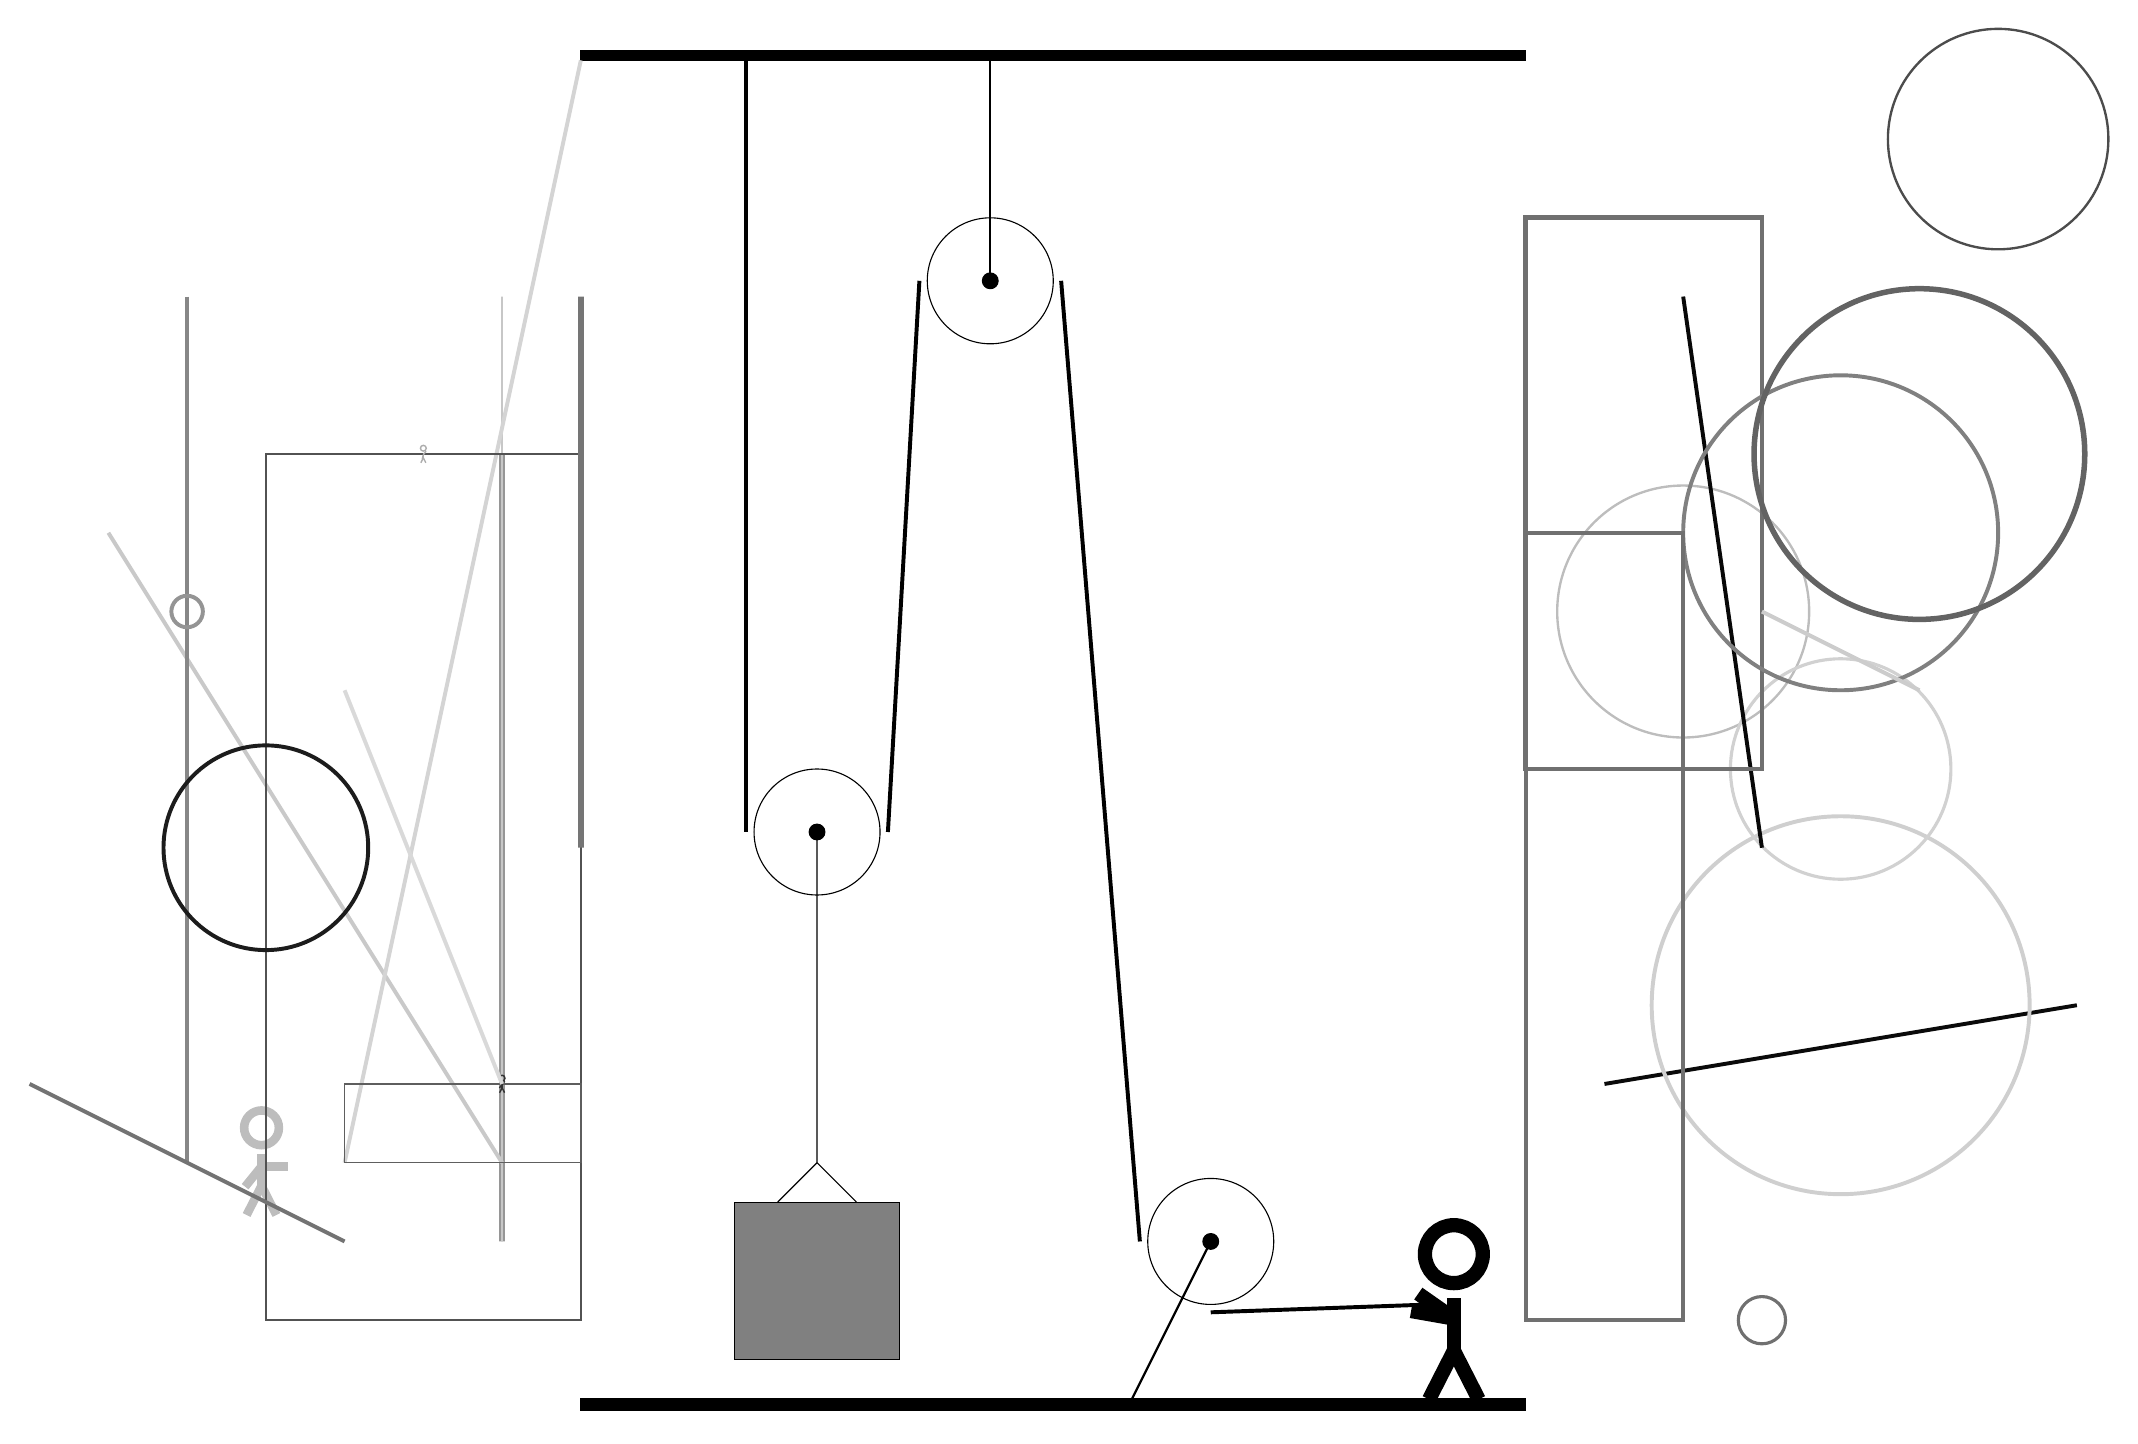
\begin{tikzpicture}
			%%%%% START %%%%%
			
			\draw[fill=black] (-2, 14) rectangle (10, 14.125);
			
			\draw (3.2, 11.2) circle (0.8);
			\draw[fill=black] (3.2, 11.2) circle (0.1);
			\draw[thick] (3.2, 11.2) -- (3.2, 14);
			
			\node[line width=0.2mm, color=black!26] at (-6, 0) {\Strichmaxerl[6][51][0]};
			
			\draw[line width=0.7mm, color=black!41] (-3, -1) rectangle (-3, 9);
			\draw[line width=0.5mm, color=black!21](-3, 0) -- (-8, 8);
			\draw [line width=0.3mm, color=black!70](16, 13) circle (1.4);
			\draw[line width=0.3mm, color=black!22] (-3, -1) rectangle (-3, 11);
			\draw[line width=0.5mm, color=black!47](-7, 11) -- (-7, 0);
			
			\draw[line width=0.5mm, color=black!17](-5, 0) -- (-2, 14);
			\draw[line width=0.3mm, color=black!68] (-2, -2) rectangle (-6, 9);
			\draw[line width=0.2mm, color=black!63] (-2, 1) rectangle (-5, 0);
			\draw[line width=0.5mm, color=black!96](11, 1) -- (17, 2);
			\node[line width=0.2mm, color=black!32] at (-4, 9) {\Strichmaxerl[1][76][52]};
			
			\draw[line width=0.7mm, color=black!54] (-2, 4) rectangle (-2, 11);
			\draw [line width=0.3mm, color=black!26](12, 7) circle (1.6);
			
			\draw [line width=0.5mm, color=black!19](14, 2) circle (2.4);
			\draw[line width=0.5mm, color=black!55](-5, -1) -- (-9, 1);
			\draw [line width=0.4mm, color=black!56](13, -2) circle (0.3);
			\draw [line width=0.4mm, color=black!18](14, 5) circle (1.4);
			
			\draw[line width=0.5mm, color=black!97](12, 11) -- (13, 4);
			\draw[line width=0.6mm, color=black!56] (10, 12) rectangle (13, 5);
			\draw [line width=0.5mm, color=black!89](-6, 4) circle (1.3);
			\draw [line width=0.5mm, color=black!50](14, 8) circle (2.0);
			
			\node[line width=0.2mm, color=black!80] at (-3, 1) {\Strichmaxerl[1][51][53]};
			\draw[line width=0.5mm, color=black!56] (12, -2) rectangle (10, 8);
			\draw [line width=0.5mm, color=black!42](-7, 7) circle (0.2);
			\draw [line width=0.7mm, color=black!61](15, 9) circle (2.1);
			
			\draw[line width=0.5mm, color=black!15](-5, 6) -- (-3, 1);
			\draw[line width=0.5mm, color=black!20](13, 7) -- (15, 6);
			
			\draw (6, -1) circle (0.8);
			\draw[fill=black] (6, -1) circle (0.1);
			\draw[thick] (6, -1) -- (5, -3);
			
			\draw (1, 4.2) circle (0.8);
			\draw[fill=black] (1, 4.2) circle (0.1);
			
			\draw (1, 4.2) -- (1, 0) -- (0.5, -0.5);
			\draw (1, 0) -- (1.5, -0.5);
			\draw[fill=black!50] (-0.05, -0.5) rectangle (2.05, -2.5);
			
			\draw[line width=0.5mm] (0.1, 14) -- (0.1, 4.2);
			\centerarc[line width=0.5mm](1, 4.2)(180:360:0.9);
			\draw[line width=0.5mm](1.9, 4.2) -- (2.3, 11.2);
			\centerarc[line width=0.5mm](3.2, 11.2)(0:180:0.9);
			\draw[line width=0.5mm](4.1, 11.2) -- (5.1, -1);
			\centerarc[line width=0.5mm](6, -1)(180:270:0.9);
			\draw[line width=0.5mm](6, -1.9) -- (8.8, -1.8);
			
			\node at (9, -1.9) {\Strichmaxerl[10][-35][170]};
			
			\draw[fill=black] (-2, -3) rectangle (10, -3.15);
			
			%%%%% END %%%%%
		\end{tikzpicture}
	\end{figure}	
\end{document}